\documentclass[15pt,twoside]{report}
\usepackage[utf8]{inputenc}


\usepackage[a4paper,width=150mm,top=25mm,bottom=25mm,bindingoffset=6mm]{geometry}
\usepackage[british]{babel}
\usepackage{csquotes}

\usepackage{graphicx}
\usepackage{float}
\usepackage{fancyhdr}
\usepackage[nohyperlinks, printonlyused, withpage, smaller]{acronym}
\usepackage[backend=biber, sorting=nyt, style=ext-authoryear-comp,dashed=false,block=par]{biblatex}
\usepackage[inkscapeformat=png]{svg}
\usepackage{booktabs,multirow,array}
\usepackage{listings}
\usepackage{xcolor}
\usepackage{amsmath}

\usepackage[font=small,labelfont=bf,tableposition=top]{caption}
\usepackage{tikz}
\usepackage{tocloft}
\usepackage{enumitem}
\usepackage{appendix}
\usepackage{mathrsfs}

% \title{\Large \textbf{Application of Natural Language Processing \\ and Machine Learning in E-Commerce} \\ \Large Predicting Product Taxonomy}
\usetikzlibrary{shapes,arrows,positioning,arrows.meta,calc}
\captionsetup[table]{skip=5pt}

% Customize list of figures appearance in table of contents
\renewcommand{\cftfigpresnum}{\figurename\ }
\setlength{\cftfigindent}{0pt}
\setlength{\cftfignumwidth}{6.5em}


\definecolor{codegreen}{rgb}{0,0.6,0}
\definecolor{codegray}{rgb}{0.5,0.5,0.5}
\definecolor{codepurple}{rgb}{0.58,0,0.82}
\definecolor{backcolour}{rgb}{0.95,0.95,0.92}




% Define the page style "mystyle" for the fancyhdr package
\fancypagestyle{mypagestyle}{
     % Clear all header and footer fields
     \fancyhf{}
     % Set the header to display the chapter name on the right side
     \fancyhead[R]{\leftmark}
     % Set the footer to display the page number on the center
     \fancyfoot[C]{\thepage}
     % Set the footer line to appear (change 0pt to desired line thickness)
     \renewcommand{\footrulewidth}{0.4pt}

}

\lstdefinestyle{mystyle}{
    backgroundcolor=\color{backcolour},   
    commentstyle=\color{codegreen},
    keywordstyle=\color{magenta},
    numberstyle=\tiny\color{codegray},
    stringstyle=\color{codepurple},
    basicstyle=\ttfamily\footnotesize,
    breakatwhitespace=false,         
    breaklines=true,                 
    captionpos=b,                    
    keepspaces=true,                 
    numbers=left,                    
    numbersep=5pt,                  
    showspaces=false,                
    showstringspaces=false,
    showtabs=false,                  
    tabsize=2
}

\lstset{style=mystyle}

\graphicspath{ {images/} }

% \renewbibmacro*{url+urldate}{%
%   \printfield{url}%
%   \iffieldundef{urlyear}
%     {}
%     {\setunit*{\addspace}%
%      \printtext[urldate]{\printurldate}}}

\DeclareFieldFormat{url}{Available at\addcolon\space\url{#1}}
\DeclareFieldFormat{urldate}{\newline Accessed on\addcolon\space{#1}}
% \DeclareFieldFormat{title}{\newline{#1}}
\DeclareFieldFormat{biblabeldate}{#1}
\DeclareDelimFormat{nameyeardelim}{\addcomma\space}% comma before the year
% \DeclareFieldFormat{url}{\bibstring{urlfrom}\addcolon\space\url{#1}}
% \DeclareFieldFormat{urldate}{\mkbibbrackets{\bibstring{urlseen}\addcolon\space#1}}

% \renewbibmacro*{url+urldate}{% changes the default order of the fields url and urldate
%                              \usebibmacro{urldate}%
%                              \newunit
%                              \usebibmacro{url}%
%                             }

%                             \makeatletter
%                             \setlength{\bibitemsep}{0.5\baselineskip plus 0.5\baselineskip}
                            
%                             \newsavebox\ay@labelbox
%                             \newlength{\labwidthsameline}
%                             \setlength{\labwidthsameline}{6em}
                            
%                             % \newbibmacro{labelwidthbib}{%
%                             %   \begingroup
%                             %   \delimcontext{parencite}%
%                             %   \DeclareFieldFormat{bibhyperref}{##1}%
%                             %   \csuse{blx@hook@cite}%
%                             %   \csuse{blx@hook@citekey}%
%                             %   \global\undef\cbx@lasthash
%                             %   \global\undef\cbx@lastyear
%                             %   \citetrackerfalse\pagetrackerfalse\backtrackerfalse
%                             %   \defcounter{maxnames}{\blx@maxcitenames}%
%                             %   \printtext[brackets]{\usebibmacro{cite}}%
%                             %   \endgroup
%                             % } 
%                             %-----------------------
%                             \newbibmacro{kicklabel}{% 
%                               \sbox\ay@labelbox{\usebibmacro{labelwidthbib}}%
%                               \global\togglefalse{blx@insert}%
%                               \ifdim\wd\ay@labelbox>\labwidthsameline
%                                 \leavevmode\newline
%                               \fi
%                             }
                            
%                             \defbibenvironment{bibliography}%
%                               {\list
%                                 {\usebibmacro{labelwidthbib}}%
%                                 {\setlength{\labelwidth}{\labwidthsameline}%
%                                  \setlength{\leftmargin}{\labelwidth}%
%                                  \setlength{\labelsep}{\biblabelsep}%
%                                  \addtolength{\leftmargin}{\labelsep}%
%                                  \setlength{\itemsep}{\bibitemsep}%
%                                  \setlength{\parsep}{\bibparsep}%
%                                  \renewcommand*{\makelabel}[1]{##1\hss}}}%
%                               {\endlist}%
%                               {\item\usebibmacro{kicklabel}}
%                             \makeatother

\addbibresource{References.bib}

\includeonly{preliminary/title, %
preliminary/affidavit, %
preliminary/abstract, %
preliminary/acronyms, %
chapters/introduction, %
chapters/literature-review, %
chapters/data-preprocessing, %
chapters/model-selection, %
chapters/training-hypertuning, %
chapters/math-behind, %
chapters/building-kg, %
chapters/conclusion, %
chapters/appendix%
}

\begin{document}


%--------------- Prelimanary pages -------------


%--------------------------------------------
\begin{titlepage}

    \vspace*{3\baselineskip}
        \begin{flushright}        
  
                \includegraphics[scale=0.3]{SRH_Hochschule_Heidelberg_logo.svg.png}
           
        \end{flushright}
    \vspace*{3\baselineskip}

    \centering
   


    {\Large \bfseries Application of Natural language processing in E-Commerce \\ Predicting product taxonomy}
    \vspace*{3\baselineskip}

    {\Large Master Thesis}
    \vspace*{1\baselineskip}

    {\Large by }
    \vspace*{2\baselineskip}

    {\Large  \bfseries Shoney Arickathil }
    \vspace*{0.5\baselineskip}

    {\Large  Student no: 11017678 }
    \vspace*{2\baselineskip}

    {\Large \today}
    \vspace*{8\baselineskip}

    % \includegraphics[width=0.35\linewidth]{srhlogo}

    {\Large  Masters in Applied Computer Science }
    \vspace*{0.5\baselineskip}

    {\Large  SRH University Heidelberg \\ School of Informatics}  
    \vspace*{6\baselineskip}

    \begin{minipage}{\textwidth}
        \begin{flushleft} % Left-align supervisor's name
            \large Primary Supervisor: \hfill \bfseries Prof. Dr. Gerd Moeckel
           
        \end{flushleft}
       
       
    \end{minipage}

    


   
    
\end{titlepage}

\begin{titlepage}
    \begin{flushright}
        
  
\section*{Declaration}
\justifying{
I hereby declare that the work presented in this Project Report titled \textbf{ Machine Learning for traffic flow prediction at different junctions – M.Tech}. Submitted to the \textbf{ Indian Institute of Technology Jodhpur} in partial fulfilment of the requirements for the award of the degree of M.Tech (Masters of Technology), is a Bonafide record of the research work carried out under the supervision of \textbf{ Dr. Ranju Mohan}. The contents of this Project Report in full or in parts, have not been submitted to, and will not be submitted by me to, any other Institute or University in India or abroad for the award of any degree or diploma.
}
\vspace*{3\baselineskip}


{\large \bfseries Cyril John Arickathil \par}
{\large \bfseries M22RM210 \par}


\end{flushright}

\end{titlepage}

\chapter*{Abstract}
An abstract is a concise summary of a research paper or entire thesis. It is an original work, not an excerpted passage. An abstract must be fully self-contained and make sense by itself, without further reference to outside sources or to the actual paper.



\pagenumbering{roman}
\pagestyle{plain}
\tableofcontents

\clearpage
%----------------- chapters --------------------
\pagestyle{mypagestyle}
\pagenumbering{arabic}

%---------------------------------------
\chapter{Introduction}

\section{Topic overview}

While working at an E-commerce company selling automobile parts, author realized that various manufacture and suppliers of similar kind of automobile parts may have different product taxonomy. Defining the product taxonomy is a prior task of product deployment. Manually defining the product taxonomy requires a significant amount of time and are prone to error. \\

E-commerce industry is growing, and many products are sold online. Use of machine learning model for suggesting the products to the customer, auto completing the search text, auto filtering of products based on the text provided by the user describing the product are few of the tasks which is managed by artificial intelligence. All the tasks can only be performed appropriately only if the product taxonomy is well-defined. \\

 

\section{Problem statement and Research question}

\begin{itemize}
    \item RQ1: How to define product features as an input for machine learning model?
    \item RQ2 : Which type of neural network is the best suitable for text classification in terms of product classification?
    \item RQ3 :  How should the model parameters be defined to optimize the neural network?
\end{itemize}

\section{Methodology}

Machine learning model to text classification for predicting the product taxonomy is a methodology in which a lot of research have been conducted \parencite{AliCevahir.} \parencite{Gupta.20062016}. In this thesis, author classifies the product by representing the features of the product into vector of entire vocabulary of dataset. This approach is inspired by \parencite{sean}, in which the language of the name is predicted based on the pattern of characters in name input. 

\section{Thesis structure}

In the first chapter, gives the introduction of the thesis along with research questions and methodology.

In the second chapter, defining or selecting the features from a document is described. It introduces various analytic engine tools and methods for feature selection. 

The third chapter describes various methods to standardize the text data and preprocess it before making it as an input to the classification model.

The fourth chapter focuses on retaining the missing textual data from the dataset from which the classification model will be predicting the product category. 

The fifth chapter is a guideline on vectoring or transforming the text into machine usable numerical form called feature extraction.

In the sixth chapter, how author classifies the product by representing the features of the product into vector of entire vocabulary of dataset is depicted. The architecture of neural network used for the prediction is described in this chapter. Mathematical equations on probability distribution, Softmax and why to apply log to softmax is formulated. 

In the seventh chapter, the model is trained to classification. The experimentation and analysis of model with different approaches and varying model parameters is conducted.

The eight chapter, is research on creating a knowledge graph with natural language processing.
\chapter{Literature Review}

\section{E-commerce and Product Taxonomy}

A product taxonomy is a hierarchical representation of product catalog organized logically so that the customer can find the product in the fewest possible clicks. The top levels of hierarchy are general terms and low levels are narrowed down to specific and semantically closer to the product.  


In figure \ref{fig:sample-product-taxonomy}, is a sample of product taxonomy represented in a \acf{DAG}.

\begin{figure}[H]
    \centering
    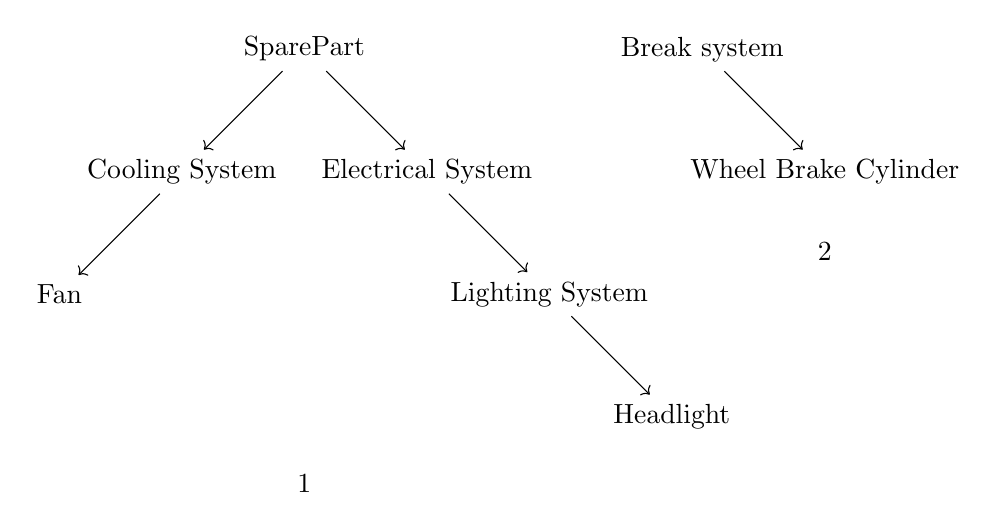
\begin{tikzpicture}[node distance=2.2cm]
        % Nodes
        \node (sparepart) {SparePart};
        \node (break-system)[right=3cm of sparepart] {Break system};
        \node (cylinder-head)[below right of=break-system] {Wheel Brake Cylinder};
        \node (coolingsystem) [below left of=sparepart] {Cooling System};
        \node (fan) [below left of=coolingsystem] {Fan};
        \node (electricalsystem) [below right of=sparepart] {Electrical System};
    
        \node (lightingsystem) [below right of=electricalsystem] {Lighting System};
    
        \node (headlighgt) [below right of=lightingsystem] {Headlight};

        \node (one) [below =5cm of sparepart] {1};
        \node (two) [below =0.5cm of cylinder-head] {2};
        
        % Arrows
        \draw[->] (sparepart) -- (coolingsystem);
        \draw[->] (coolingsystem) -- (fan);
        \draw[->] (sparepart) -- (electricalsystem);
        \draw[->] (electricalsystem) -- (lightingsystem);
        \draw[->] (lightingsystem) -- (headlighgt);
        \draw[->] (break-system) -- (cylinder-head);
      \end{tikzpicture}
      \caption{Sample - Product taxonomy}
      \label{fig:sample-product-taxonomy}
     
\end{figure}

\begin{enumerate}[label=\textbf{Q\arabic*:}]
    \item What are the characteristics of sample of product taxonomies illustrated in figure \ref{fig:sample-product-taxonomy}?
    

    \begin{itemize}
        \item The top level of root node traversing below to leaf nodes connected with unidirectional edges representing hierarchical levels between the nodes. 
        \item Product taxonomy has different lowest levels of hierarchy. For example, category ``Fan'' is at third level and ``Headlight'' being a part of ``Electrical Systems'' is at fourth level.
        \item Few categories having similar vocabulary are part of same graph. For example, category with the word ``Brake'' are connected with the edges.  Similarly, the category ``Lighting system'' and its leaf node ``Headlight'' share the same prefix or suffix word ``light''.
        \item The root nodes ``Sparepart'' and ``Break system'' are isolated from each other.  
        \item The node ``Break system'' could also be a part of node ``Sparepart'' and yet the taxonomy will remain well-defined as it is a general term.
        
    \end{itemize}
    
    \clearpage
    
    \item How important is a well-defined product taxonomy in e-commerce \parencite{JessicaHoward.}?
    \begin{itemize}
        \item \textbf{Simplify product searches}:\\ Customer filters the categories to narrow down the search result, enabling them to find the required product in the fewest possible clicks. This improves customer experience.
        \item \textbf{Better product recommendation}:\\ Product recommendation system analyze the customer behavior and returns the related products. Customer behavior such as to know which category the customer clicked on but did not purchase the product yet, enabling recommendation of most relevant products. 
        \item \textbf{Improves search engine optimization (SEO)}:\\  Organizing the products into structured taxonomy, businesses can ensure that their products are found easily. It also helps business drive more organic traffic. 
    \end{itemize}
    \item What are the challenges in defining the product taxonomy?     

    \begin{itemize}
        \item \textbf{Scalability}:\\ The taxonomy requires to be able to update as the number of products in a business grows.
        \item \textbf{Internationalization}:\\ Multi lingual taxonomy is required to reach out to customers internationally. 
        \item \textbf{Product complexity}:\\  Some products may have multiple attributes and these needs to be taken into account while creating the taxonomy. This process can complicate the process.
        \item \textbf{Changing product}:\\ Taxonomy of product need to regularly updated as and when there is a change in product. 
    \end{itemize}

\end{enumerate}

\section{\acf{PIM}}
\acl{PIM} system is an information system that facilitates the manufactures and distribution channel such as an e-commerce website with a central hub of product data \parencite{iceclog}. \acs{PIM} system manages products details such name, description, manufacturer, price as well as the products' taxonomy. A PIM system may also include the \acf{SKU}. \acsp{SKU} enables the distribution channels to determine which product require reordering and also provides sales data. Distribution channels may also have an extended version of the \acs{SKU} than the one provided by the suppliers.

\acsp{PIM} are the point of source to verify whether the products' taxonomy are correct and also if the stock is available before distribution channels make it publically available for sales.


% \begin{tikzpicture}[
%     node distance=1cm,
%     every node/.style={font=\footnotesize},
%     arrow/.style={->,>=Stealth},
%     process/.style={rectangle, draw, text centered, minimum width=2.5cm, text width=2.5cm},
%     decision/.style={diamond, draw, text centered, aspect=2},
%     arrowlabel/.style={midway, above, font=\scriptsize},
% ]
%     % Define nodes
%     \node (dc) [process] {Distribution Channels};
%     \node (dp) [process, below=3cm of dc] {Available for Sale};
%     \node (ms) [process, right=6cm of dc] {Source};
%     \node (pim) [process, right=3cm of dc, yshift=-1.5cm] {PIM System};
%     \node (check) [decision, below=of dc] {Verify};
   
%     % Define arrows and labels
%     \draw [arrow] (dc) -- (check);
%     \draw [arrow] (check) -- node[arrowlabel] {Yes} (dp);
%     \draw [arrow] (check.east) -- node[anchor=south] {No} ++(1.5,0) |- ($(pim.west) + (0,0.5)$) -- (pim.west);
%     \draw [arrow] (ms) -- (pim.east) ; 
%     \draw [arrow] (pim.north) -- (dc.east);
% \end{tikzpicture}


% \begin{itemize}
%     \item Getting updated lists of products from suppliers.
%     \begin{itemize}
%         \item What is the current method to get the updates?
%         \item In which cycle do these updates occur? Is it the same cycle for every supplier or is it individual?
%     \end{itemize}
%     \item Best way to activate / deactive products.
%     \begin{itemize}
%         \item Would it make sense to have article level toggles in the interface that will (de)activate a product from the Reorder?
        
%         \item Would a standardised document import be a better solution?
%     \end{itemize}
% \end{itemize}






\section{Product Taxonomy Prediction Approaches}


A lot of research have been conducted on methodology for predicting taxonomy. Prediction of taxonomies narrows down to text classification. Text classification is a process of identifying the group or category in which the  text belongs to.  Few classification methods are decision trees, naive Bayes classifier and max entropy classifiers \parencite{BirdKleinLoper09}. 


\begin{itemize}
    \item Decision  tree
    
    A decision tree is a flowchart that selects labels for input values. This flowchart consists of decision nodes, which check feature values, and leaf nodes, which assign labels. 

    \item Naive Bayes classifiers
    
    In naive Bayes classifiers, each feature values determining which label should be assigned to a given input value. It begins by calculating prior probability of each label. It is determined by frequency of each label in the training set. Upon combining these prior probability, the likelihood estimation is calculated for each label. The with the highest likelihood estimate is assigned to the input values.


    \begin{figure}[H]
        \centering    
        \includegraphics[scale=0.7]{naive_bayes_bargraph.png}
        \caption{Calculating label likelihoods with naive Bayes \parencite{BirdKleinLoper09}}
        \label{fig:Calculating label likelihoods with naive Bayes}
    \end{figure}

    \item Max Entropy
    
    Like the naive Bayes model, the Maximum Entropy classifier calculates the likelihood of each label for a given input.
    However, Maximum Entropy classifier model leaves it up to the user to decide what combinations of labels and features should receive their own parameters.

\end{itemize}

\clearpage

\section{Supervised Learning}

The machine learning model built using existing dataset is called supervised learning. ´Figure \ref{fig:sup learinig workflow} illustrates the supervised learning workflow. In this paper, author builds a supervised learning model to predict the product taxonomies. The work flow starts with data collection, this steps involves fetching the corpus of raw data. This raw data processed before creating a training data set out of it. The data preprocessing steps involves feature selection, text normalization, data imputation and feature extraction. The training data is passed an input to the model which compares its results with the actual value to self evaluate and learn. If any hyperparameter tuning for the machine learning model is required then it is trained again with new parameters. The model is then evaluated and then deployed for production use.

\begin{figure}[H]
    \centering
    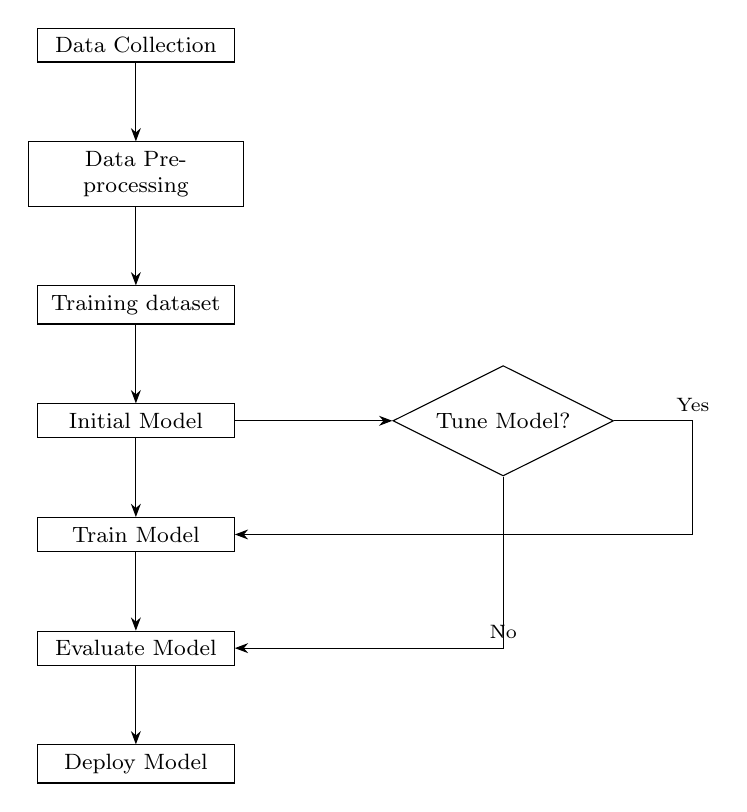
\begin{tikzpicture}[
        node distance=1cm,
        every node/.style={font=\footnotesize},
        arrow/.style={->,>=Stealth},
        process/.style={rectangle, draw, text centered, minimum width=2.5cm},
        data/.style={rectangle, draw, text centered, text width=2.5cm},
        decision/.style={diamond, draw, text centered, aspect=2},
        arrowlabel/.style={midway, above, font=\scriptsize},
    ]
        % Nodes
        \node (start) [process] {Data Collection};
        \node (data) [data, below=of start] {Data Preprocessing};
        \node (split) [process, below=of data] {Training dataset};
        \node (model) [process, below=of split] {Initial Model};
        \node (train) [process, below=of model] {Train Model};
        \node (evaluate) [process, below=of train] {Evaluate Model};
        \node (deploy) [process, below=of evaluate] {Deploy Model};
     
        
        % Arrows
        \draw [arrow] (start) -- (data);
        \draw [arrow] (data) -- (split);
        \draw [arrow] (split) -- (model);
        \draw [arrow] (model) -- (train);
        \draw [arrow] (train) -- (evaluate);
        \draw [arrow] (evaluate) -- (deploy);

        
        % Decision point
        \node (decision) [decision, right=of model, xshift=1cm] {Tune Model?};
        \draw [arrow] (model) -- (decision);
        \coordinate[right=of decision] (temp);
        \draw [arrow] (decision) -| node[arrowlabel] {Yes} (temp) |- (train);
        \draw [arrow] (decision) |- node[arrowlabel] {No} (evaluate);
    \end{tikzpicture}
    \caption{Supervised Learning Workflow}
    \label{fig:sup learinig workflow}
\end{figure}


\section{Related Works}

\parencite{AliCevahir.} describes implementing classification model by chunking the process to predict at every level using the \acl*{KNN} classifier. \parencite{Gupta.20062016}  proposes a distributional semantics representation for predicting the product taxonomies.

\subsection*{Facet Suggestion}


\parencite{Tagliabue.26052020} proposes a machine learning encoder-decoder model architecture that generates the path in catalog taxonomy in real time. This model predicts the best facets - i.e. product categories in real time during type ahead on a eCommerce website search bar. In \parencite{Tagliabue.26052020} work, prediction is based on user personalized model provided with shopping session and user queries. Combining linguistic and behavioral in-session data, narrows down the search results with personalized facet prediction as shown in figure \ref{fig:Personalized facet prediction}. 




\begin{figure}[H]
    \centering    
    \includegraphics[scale=0.7]{facet2.png}
    \caption{Personalized facet prediction. \parencite{Tagliabue.26052020}}
    \label{fig:Personalized facet prediction}
\end{figure}


\subsection*{Learning to Rank}

Learning to rank is a machine learning algorithm for \acf{IR}. The application of \acf{LTR} model in E-Com is to list most relevant products based on the search query. 

\parencite{KarmakerSantu.2017} uses LambdaMART \parencite{burges2010from} as  \acs{LTR} model as it is well known to work with Web search. As per \parencite{KarmakerSantu.2017}, E-Com search logs contain four prominent relevance feedback signals.

\begin{itemize}
    \item clicks : Computed as the ratio of clicks a product receives for a query and its impressions (number of times shown to the user) for the query.
    \item cart-adds: Computed as the ratio of add-to-carts a product receives for a query and its number of clicks for the query.
    \item orders: Computed as the ratio of orders a product receives for a query and its impressions for the query.
    \item revenue: Computed as the ratio of revenue generated by a product for a query and its impressions for the query.

\end{itemize}

\parencite{KarmakerSantu.2017} proposes an algorithm based on the statistics of feedback signals to rank the relevance of product. 


\subsection*{Conversational commerce}

 Conversational commerce is a way of businesses to interact with customers using chatbots. \parencite{ChrisMessina} inventor of the hashtags, coined the term conversational commerce. In his post, he states that ecommerce will experience transformation, with integration of \acf{AI} specialized in complex task of online shopping and product research.  Conversational commerce offers convenience, personalization and decision support while people are on the go and cannot pay full attention.  
 
 One of the use case of conversational commerce is in the reverse logistics- return and exchange. For example, if the user has ordered and wrong product and would like to return it while being on the go. He may use the chatbot assistance and type "I want to return." The chatbot lists the delivered products list and customer selects the product to be returned. 

Application of knowledge graphs within the e-commerce industry involves the creation of network of information concerning the products. This knowledge graph can serve as the basis for chatbots to provide answers to user queries. 
\chapter{Data Preprocessing}

\section{Feature Selection}

Data collection is simply a process of fetching the data from the data source. However, feature selection is a process of selecting fields from which the target field will be predicted. Suppliers provide stock details along with associated product taxonomy. Importing well-defined taxonomy requires to train the classification model with already existing correct pair of features and label. The already existing pair of features and the correct label for each input is the training data set or training corpora. The classifier built on such a training corpora is termed as supervised classification \parencite{BirdKleinLoper09}.

\begin{figure}[H]
      \centering    
      \includegraphics[scale=0.9]{supervised-classification.png}
      \caption{Supervised classification \parencite{BirdKleinLoper09}}
      \label{fig:supervised-classification}
  \end{figure}

  As illustrated in figure \ref{fig:supervised-classification}, during training, a pair of feature set and label are fed in to the machine learning algorithm to generate a classifier model. During prediction, same feature set are fed into the model to predict the label. Refer to chapter \ref{ch:feature-extraction} for details on feature extraction.

In this project, author choose to create a classification model with only one feature that is the name of the product. However, author identifies the potential features to classify the target of n levels of category. These features have been identified based on the understanding of domain of the product. For products with many details will have many more features to be taken into consideration. In such case, selection based on common understanding of the nature of the product may not be sufficient. Hence, Scikit learn  \parencite{sklearn_api} provides methods to define feature appropriately. 


\subsection {Feature Selection Methods} \label{sec:feature-selection}

A feature represents a dataset fine-tuned to serve as a training data for machine learning model. Choosing obvious set of features could get a decent performance on classification task. However, carefully constructed relevant set of features could impact the learning ability and have a significant gain in performance. The feature selection API from Scikit learn \parencite{sklearn_api} also refers to it as dimensionality reduction. 

\parencite{BirdKleinLoper09}  describes some approaches for feature selection as following:

\begin{itemize}
      \item Kitchen sink 
      

      All the features are initially included later each are checked to determine whether they are actually helpful.

      \item Error analysis
      
      The data corpus is split into development-set and test-set. Development-set is subdivided into training set and dev-test set. Training set is used to train the model, dev-test set is employed for error analysis.  The individual error cases are examined for wrongly predicted labels.
      
      
      \begin{figure}[H]
            \centering    
            \includegraphics[scale=0.5]{corpus-org.png}
            \caption{Corpus organization for supervised classification \parencite{BirdKleinLoper09}}
            \label{fig:corpus-supervised-classification}
        \end{figure}

\end{itemize}

 Methods for feature selection with Scikit Learn API are:-
\begin{itemize}
      \item Removing features with low variance
      \item Univariate feature selection
      \item Recursive feature elimination

\end{itemize}

\subsection{Obvious Feature Selection}

In this paper, the datasets used are of an ecommerce business specializing in automotive industry domain. Secondary dataset used is from the TecDoc catalogue by TecAlliance \footnote{https://www.tecalliance.net/}. 

Table \ref{table:feature_decription} lists the obvious features for an ecommerce domain. In this paper, five levels of categories are taken into consideration. The number of category levels differ for each product. Consider an example of category tree with three levels. 

\begin{quote} 
\centering 
sparepart/cooling-system/thermostat
\end{quote}
In this example, the lowest level of category is ``thermostat'' as level 4 and level 5 does not exist and will be represented by black or NaN. These blank or NaN value records can go through data imputation as discussed in chapter \ref{ch:data-imputation}.



\begin{table}[h]
      \centering
      \caption{Feature description}
      \label{table:feature_decription}
      \begin{tabular}{ lll }
            \toprule
            
            \textbf{No}& \textbf{Feature} & \textbf{Description}\\
            \midrule
            1&Product name & normalized form of name\\
            2&Category tree & multi level categories\\
            3&Description & Description with html tags\\         
            4&Short description  & product info displayed\\
            5&Supplier  &  supplier of the product\\
            6&Manufacturer  &  manufacturer of the product\\           
            7&Price  &  Price of the product\\
            8&Dimension  & Height, weight of the product\\
            9&(n-1) number of  category levels   &  n is the total category level, one of which will be the target\\
           
            \bottomrule
            \end{tabular}


\end{table}

\subsection {Fetch Existing Product Taxonomy (Corpus) using Elasticsearch}
Elastic search \footnote{https://www.elastic.co/} is a fast and scalable search and analytics engine. It can build a powerful AI and machine learning enabled search experience. In this paper, author fetches labeled dataset of products to serve as the training data for the machine learning model.
For this project, python client elasticsearch 6.8.2 is installed as the client needs to be compatible with Elastic search version being used. The official Python client provides mapping with Elasticsearch REST APIs.

\begin{lstlisting}[language=Python]
resp=self.es.search("english-name-category",{"_source":["id","name","category"],
'from':_from,
'size' :_size ,
"query": {"match_all": {}}})
\end{lstlisting}

The above code fetches indexed product name and its lowest hierarchy level category.  
\begin{table}[h]
      \caption{Index: english-name-category statistics}
      \centering
      \label{table:enc}
\begin{tabular}{ll}
      \toprule 

      Samples total&22160 \\
      Dimensionality&2 \\
      Features&name \\
      Label&category \\
      
      \bottomrule
\end{tabular}
\end{table}

Table \ref{table:enc} highlights the total number of products and category and name of fields considered as feature and label. 

\section{Text Normalization} \label{text_normalization}

Text normalization is a process of transforming the document into a standard and consistent form of a text. A document is a text from single source. Some examples of document are list of product names from databases, a pdf file, texts retrieved from web scraping. Text normalization enables to perform required operations on the text as the text inputs are consistent across the document. The process of text normalization varies based on the type of text that needs to be normalize. There is no standard method for text normalization task. In this paper, text normalization of product name and category from the database source is performed. 

In table \ref{table:TN}, displays the difference in text before and after normalization. 

\begin{table}[h]
      \caption{Sample of text normalization effect}
      \centering
      \label{table:TN}
\begin{tabular}{lll}
      \toprule 
                  &\textbf{Name} & \textbf{Category} \\ 
      \midrule
      \textbf{Before}& Company V10-4245 Stoßdämpfer & Stoßdämpfer \\
      \textbf{After}&company v104245 stossdaempfer & stossdaempfer \\
      
      \bottomrule
\end{tabular}
\end{table}

\subsection{Lower Case Conversion}

Using Pandas - vectorized string method, a text can be lower cased across the document. These methos exclude the missing  / NA values automatically \parencite{mckinney-proc-scipy-2010}.

\begin{lstlisting}[language=Python, caption={Pandas vectorized string method }]
      df_de["name"]= df_de["name"].str.lower()
\end{lstlisting}

\subsection{HTML Parsing}

Probability of getting html tags in a document increases if the source of document is from web scraping or also if the document from database source has inline html tags. In such case, fetching normal texts from a html text is required. One of the method would be to use regular expressions to get text in between angel brackets \textless \textgreater text \textless \textgreater. However, this method would require to have the tags to be well formed.
\begin{lstlisting}[language=Python, caption={Regular expression to get text from html}]
      text = re.sub('<[^>]*>', '', text)
\end{lstlisting}



The better option would be to use Beautiful Soup \footnote{https://www.crummy.com/software/BeautifulSoup/bs4/doc/} a Python library for pulling data out of HTLM and XML.
\begin{lstlisting}[language=Python, caption={Beautiful soap API to get text from html}]
      # Remove html tags 
      soup = BeautifulSoup(doc, 'html.parser')
      text =soup.get_text()
\end{lstlisting}

\subsection{Cleaning Text}
A product detail text may contain non-word characters represented in regular expression as \textbackslash W. It may also contain space separated decimals describing the dimensional values of the product such as weight, height. Regular expressions could be used for removing the non-character words and spaces between the decimal values. 

\begin{lstlisting}[language=Python,,caption={Clean text with Regular expression}]
      text = (re.sub('[-\W]+', ' ', text))
      text = (re.sub('(?<=\d) (?=\d)', '', text))
\end{lstlisting}

\subsection{Normal form D - Unicode database}

A product name in Deutsch language may contain umlaute characters such as \"A.  Pythons unicodedata \footnote{https://docs.python.org/3/library/unicodedata.html} module provides access to the Unicode Character Database (UCD) which defines the character properties for all Unicode characters. To change \"A to A, the Normal form D (NFD) should be applied which translated each character into its decomposed form. Further the text can be refined with the general category assigned to the character as string. Nonspacing mark characters \footnote{https://www.compart.com/en/unicode/category/Mn} are represented as "Mn". These characters could be removed by referring the character category.
\begin{lstlisting}[language=Python ,caption={NFD normalization}]
      ''.join(
            c for c in unicodedata.normalize('NFD', text)
            if unicodedata.category(c) != 'Mn')
\end{lstlisting}

Another option is to replace the German characters to equivalent English sounding characters. Table \ref{table:deu-eng} lists the common German characters and their equivalent English sounding series of characters. In this way, the reverse translation is easier.
\begin{table}[h]
      \centering
      \caption{German characters to English}
      \label{table:deu-eng}
      \begin{tabular}{ llll }
            \toprule
            \"A& Ö&  Ü&ß \\
            Ae&Oe & Ue&ss\\         
          
            \bottomrule
            \end{tabular}
  \end{table}


  \subsection{Avoided normalization processes}

  In this project, some commonly practiced normalization process are being avoided. Which once and why are described below.

  \begin{itemize}
      \item Stemming 
      
      Stemming is a process of striping off any affixes. \acl{nlp} tools such as NLTK provide stemmers. The Porter and Lancaster
      stemmers follow their own rules for stripping affixes \parencite{BirdKleinLoper09}. Author required not to deviate from the original vocabulary of features.

      \item Lemmatization
      
      Lemmatization remove the affixes if the word is in the used libraries' dictionary. The vocabulary for corpora and any third party library such as WordNet cannot be synced.   

  \end{itemize}



\section{Impute missing text data} \label{ch:data-imputation}

Machine leaning algorithms requires that their inputs have no missing values.
Missing values encoded as NaNs or blanks are incompatible with estimators which represents as the numerical values and assumes all values have and hold meaning. Discarding the entire row and/or columns of a dataset containing the missing values could lead to losing valuable data. The process to fill (impute) missing values are referred to as imputation.

\subsection{Feature imputation / Regression imputation or \\ Predictive Imputation}

Machine learning algorithm to predict values in a categorical variable based on other available features. Table \ref{table:feature_imputation} states the categorical features from the all the features mentioned in \ref{table:feature_decription}.


\begin{table}[h]
    \centering
    \caption{Identify categorical features}
    \label{table:feature_imputation}
    \begin{tabular}{ lll }
          \toprule
          
          \textbf{No}& \textbf{Feature} & \textbf{Categorical}\\
          \midrule
          1&Product name & No\\
          3&Description & No\\         
          4&Short description  & No\\
          5&Supplier  & Yes\\
          6&Manufacturer  &  Yes\\           
          7&Price  &  No \\
          8&Dimension  & Yes\\
          \bottomrule
          \end{tabular}
\end{table}

The \textit{dimension} column is also considered as a categorical value as it has few unique values.

If \textit{supplier} is the missing value from the set of row. The missing \textit{supplier} data must be predicted only from the available list of suppliers. A supervised machine learning with labeled dataset to train the model to classify the available features data to predict \textit{supplier}. A tensor size of the number of unique \textit{supplier} will be the output of the model. 
In an iterated round-robin fashion, at every step a missing feature column  \textit{y} and other feature columns treated as input \textit{x} predicts the missing values of \textit{y}. Regression imputation is more accurate than mode imputation on categorical value.


\subsection{Mode imputation}

Replacing the most frequent categorical value in a column is known as mode imputation.  Pandas.DataFrame.mode \parencite{mckinney-proc-scipy-2010} function returns most often value. Code snippet will fill the missing values for each column using its own most frequent value.

\begin{lstlisting}[language=Python, caption={Pandas DataFrames mode function}]
    df = df.fillna(df.mode().iloc[0])
\end{lstlisting}

Mode imputation on categorical data are prone to fill incorrect data if the missing data is not the most frequent one.



\subsection{\acf{KNN}  imputation}

\acl{KNN} is a supervised learning algorithm and is used to search dataset with the most similar elements to a given query element, with similarity defined by a distance function. This imputation method is suitable for categorical data.

The most common distance metrics functions are:-

\begin{enumerate}
    \item Euclidean distance.
    % \begin{lstlisting}[language=Python, caption={Euclidean distance formula }]
    %     dist(x, y) = sqrt(dot(x, x) - 2 * dot(x, y) + dot(y, y))
    %         \end{lstlisting}
    \item Manhattan distance.
    \item Hamming distance.
\end{enumerate}

sklearn.neighbors.KNeighborsClassifier \parencite{scikit-learn} does an instance-based learning, it does not construct a model, but stores instance of training data. Classification is computed from majority vote of nearest neighbors of each point.

The \textit{k}-neighbors classification implements learning based on  \textit{k} nearest neighbors of each query point, where \textit{k} is integer value specified by user. The optimal \textit{k} value can be evaluated by iterating the classifier with different  \textit{n\textunderscore neighbors} parameter and finding the minimum value of error rate. As per \parencite{scikit-learn}, larger \textit{k} suppresses the effects of noise, but makes the classification boundaries less distinct.

\begin{lstlisting}[language=Python, caption={Find optimal \textit{k} value in \acl{KNN} }]
    error_rate = []
    for i in range(1,40):
        knn = KNeighborsClassifier(n_neighbors=i)
        knn.fit(X_train,y_train)
        pred_i = knn.predict(X_test)
        error_rate.append(np.mean(pred_i != y_test))

    print("Minimum error:-",min(error_rate),"at K =",error_rate.index(min(error_rate)))
\end{lstlisting}



\subsection{\acs{KNN} model implementation}

In table \ref{table:KNN_implementation} there are 7 columns. Target column is \textbf{Category-Level-3} which is the category at level three.
As per the example category hierarchy in table \ref{table:KNN_implementation} 



\begin{table}[h]
    \centering
    \caption{Sample features }
    \label{table:KNN_implementation}
    \begin{tabular}{ll}
        \toprule     
        \textbf{Name}& \textit{product name} \\
        \textbf{Description}& \textit{product description} \\
        \textbf{Short-Description}& \textit{product short description} \\
        \textbf{Category-Level-1}& Spare-Part \\
        \textbf{Category-Level-2}& Cooling System \\
        \textbf{Category-Level-3}& Thermostat \\
        \textbf{Category-Level-4}& NaN \textit{product has no level 4 category} \\
        \bottomrule
    \end{tabular}

\end{table}

\begin{itemize}
    \item Collect independent data features into the X data frame and target field into a y data frame.
    \item  Split data into training and testing. 
    \item  Import the classifier model from sklearn library and fit the model with  \textit{k} value equal to the optimal value.
\end{itemize}

\begin{lstlisting}[language=Python]
    X = df.drop(['catL3'], axis = 1)
    y = df['catL3']
    from sklearn import preprocessing
    X = preprocessing.StandardScaler().fit(X).transform(X.astype(float))
    from sklearn.model_selection import train_test_split
    X_train, X_test, y_train, y_test = train_test_split( X, y, test_size=0.2, random_state=4)
    from sklearn.neighbors import KNeighborsClassifier
    from sklearn import metrics
    #Train Model and Predict
    k = 3  
    neigh = KNeighborsClassifier(n_neighbors = k).fit(X_train,y_train)
    Pred_y = neigh.predict(X_test)
    print("Accuracy of model at K=3 is",metrics.accuracy_score(y_test, Pred_y))
\end{lstlisting}



\subsection{Mean/median imputation}

Pandas.DataFrame.median \parencite{mckinney-proc-scipy-2010} returns the median value. These can be applied to the features represented in numerical value. In reference to table \ref{table:feature_imputation}, \textit{price} could be a column on which median value can be filled. However, using median to fill missing value could underestimate or overestimate the value.

\begin{enumerate}
    \item Median - The mid point value
    \item Mean - The average value
\end{enumerate}

\begin{lstlisting}[language=Python]
    df = df.fillna(df.median().iloc[0])
\end{lstlisting}

\section{Log transformation of data}

Log transformation is a mathematical operation applied on data to change its scale and to reduce its skewness and to make data more symmetric.  Skewness is a measure of the asymmetry of a distribution, and a right-skewed distribution has a long tail on the right side of the distribution \parencite{BonnieMa}.

The numpy library provides natural logarithmic function to apply log transformation on array of data.


\section{Feature extraction} \label{ch:feature-extraction}

Transforming text or image data into numerical representation usable for machine learning is called feature extraction. Raw sequence of data cannot be fed directly into a machine learning algorithm as they expect data in numerical vector and in fixed size. Whereas raw text document are of variable lengths. 

\subsection{Count Tokenization}

Tokenization is splitting the text in sequential words which can be embedded in a vector space.
For example, the normalized product name ``abc joint kit drive shaft'' can be tokenized into  ``abc'',``joint'',``kit'',``drive'',``shaft''. 

Number of occurrence of each token in a document is called counting in terms of numerical feature extraction.

\subsection{Count Vectorization or One-Hot encoding} \label{ch_countvector}


CountVectorizer class of scikit learn API implements both tokenization and occurrence counting \parencite{sklearn_api}. 

Consider a data frame with columns \textit{ProductName} and data value as in tbale \ref{table:count_vectorization}

\begin{table}[h]
    \centering
    \caption{Sample data for count vectorization}
    \label{table:count_vectorization}
    \begin{tabular}{ l }
          \toprule
          
          \textbf{ProductName}\\
          \midrule
          abc joint kit drive shaft\\
          xyz joint kit drive shaft\\
         
          \bottomrule
          \end{tabular}
\end{table}

The length of the vocabulary is the number of unique tokens in the data frame column. In the sample data the vocabulary length is six. The vector has the dimensionality equal to the size of the vocabulary. Adding one in the dimension to each of the word in the vocabulary represents one hot encoding.

\begin{table}[]
    \centering
    \caption{Sample One-Hot encoding}
    \label{table:countencode}
    \begin{tabular}{ ll }
          \toprule
          
          \textbf{text}& \textbf{encoding}\\
          \midrule
          abc&[1,0,0,0,0,0]\\
          joint&[0,1,0,0,0,0]\\
          kit&[0,0,1,0,0,0]\\
          drive&[0,0,0,1,0,0]\\
          shaft&[0,0,0,0,1,0]\\
          xyz&[0,0,0,0,0,1]\\
       
          \bottomrule
          \end{tabular}
\end{table}

\subsection{ \textit{n-grams} Vectorization} \label{sec:ngram_vector}

Count Vectorization can also be performed on range of grams of words. 

\begin{lstlisting}[language=Python,label=ngramcode, caption={\textit{n-gram} vectorization}]
    bigram_vectorizer = CountVectorizer(ngram_range=(1, 2))
    bigram_vectorizer.fit(df["ProductName"])
\end{lstlisting}


The code in listing \ref{ngramcode}, will add additional vocabularies of two words such as "drive shaft". This enables to preserve local ordering information. 

\subsection{Pickling the Vectorizer} \label{pickle_vector}

Pickle \footnote{https://docs.python.org/3/library/pickle.html} module creates a portable serialized representation of python object. Reusing the CountVectorizer object once it has been fit with the document can be enabled by Pickle module. 

\begin{lstlisting}[language=Python,label=pickle, caption={Pickle vectorization}]
    pickle.dump(self.vectorizer, open("vector.pickel", "wb"))
\end{lstlisting}

The memory use will grow as the vocabulary in the text corpus grows.  Pickling and un-pickling of vectorizer will slow for large vocabulary.
This issue can be tackled by hashing the features. 

\section{Summary}

In this chapter, search analytic engine named Elastic search is introduced. The author as a prototype of classification model choose to include only two-dimensionality. One is the feature (product name) and other is the label to be predicted (category.)

Table \ref{table:feature_decription} list the features for determining the product taxonomy. These features are listed based on general knowledge and understanding. However, productive method for refining the feature such as error analysis can be utilized for feature selection. Scikit learn API \parencite{sklearn_api} also provides some functions for feature selection.

Before extracting the features (refer chapter \ref{sec:feature-extraction}) it is important to normalize and standardize the data set. If the text normalization step is skipped then while creating the numerical representation of the text the data will be inconsistent. For example, same text with proper case (Car) or lower case (car) will have two representation even though the semantic meaning is the same.  

The methods involved in text normalization are lower casing the text, removing the HTML tags, removing irrelevant numerical data within the text such as product dimensionality, and making the text across the document with one Unicode database.

Missing input values sometimes denoted as blanks or NaN's cannot be considered for transforming into a numerical representation value. Machine learning algorithm feed in input data as a numerical representation of data terms as extracted features. Removing the missing values from the dataset sometime may not be feasible. As this may lead to loss of vital information of the product. 

Predicting the missing values, replacing the missing value with most frequent values, finding most similar value with K - nearest neighbors, replacing the values with median or mean values are some methods to replace the missing values from the dataset.


Feature extraction is a process of transforming the normalized text into numerical representation for machine learning.  Tokenization of text and Counting are terms to split the text in sequence of words and there occurrence. 

In this thesis, author has used the n-grams vectorization method to convert the feature - product name into a vector format. This creates a vocabulary of product name. For example, consider total number of unique words in entire product name column is 100. The name of the product will be a vector shape of 1 \time 100 with each text represented in one-hot encoded format. Refer table \ref{table:countencode} for visual representation.

\chapter{Defining Model Architecture: Neural networks} \label{sec:feature-extraction}

\section{Understanding Pytorch tutorial on \textit{classifying names with a character-level \acs{RNN}} } \label{sec:chRNN}

\parencite{sean} tutorial on \textit{classifying names with a character-level \acs{RNN}} provides a basic foundation for classification algorithm. In this tutorial, \Citeauthor{sean} trains on few thousand surnames from 18 languages of origin, and predicts which language the name is from based on the spelling.
\subsection{One-Hot vector representation}
\Citeauthor{sean} uses one-hot vector of size 1 x no\textunderscore letters (26 letters). A one-hot vector is filled with 0s except for a 1 at index of the letter. For example, letter b is represented as 0,1,0,0...0. To make a word, author joins a bunch of letters into 2D matrix name\textunderscore length x 1 x no\textunderscore letters.

\begin{table}[h]
    \centering
    \caption{One-Hot vector representation of name James}
    \label{table:feature_imputation}
    \begin{tabular}{ lllllllllll }
          \toprule
          
          \textbf{Letter}& \textbf{a} & \textbf{...}& \textbf{e}&\textbf{...}&\textbf{j}&\textbf{...}&\textbf{m}&\textbf{...}&\textbf{s}&\textbf{...}\\
          \midrule
          J&0 & 0& 0& 0&1& 0& 0& 0& 0& 0\\
          a&1 & 0& 0& 0&0& 0& 0& 0& 0& 0\\         
          m&0 & 0& 0& 0&0& 0& 1& 0& 0& 0\\
          e&0 & 0& 1& 0&0& 0& 0& 0& 0& 0\\
          s&0 & 0& 0& 0&0& 0& 0& 0& 1& 0\\           
        
          \bottomrule
          \end{tabular}
\end{table}
\clearpage
\subsection{Vector input and scalar output of the classification model}
It is a character level \acs*{RNN} which reads words as a series of characters. Figure \ref{fig:pytorch} shows the flow of name information to the neural network as a sequence of characters. One character at a time is feed in classification model built using RNN and outputs the language corresponding to that name.

\begin{figure}[H]
    \centering    
    \includesvg[scale=0.5]{pytorchTuitorial.svg}
    \caption{Language prediction based on name}
    \label{fig:pytorch}
\end{figure}


\section{Ideate: Vocabulary level \acs{RNN}} \label{sec:ideate}

Inspired from the character level \acs{RNN} mentioned in section \ref{sec:chRNN}, author predicts category based on the name of the products by creating a vocabulary level \acs{RNN}. As described in section \ref{ch_countvector}, product names are converted into one-hot encoded format. Vector representation of vocabulary in product name across the data frame is created. These encoded pattern of name serves as an input to the machine learning model. Model learns these patterns and predicts the category in which these patterns belong to. In section \ref{nametotensor}, the input tensors are modified to fit for use case of predicting category based on product name.  

\subsection{Convert product name to tensors} \label{nametotensor}

\begin{lstlisting}[language=Python,label=productnametotensor, caption={Convert product name to tensors},label={cd:pt}]
    def nameToTensor(self,name):
        vectorizer= pickle.load(open("vector.pickel", "rb"))
        inputSize=len(vectorizer.vocabulary_)
        vectorized=vectorizer.transform(list(name.split()))
        name_tensor=torch.zeros(1, inputSize)
        for index in vectorized.indices:
            name_tensor[0][index] = 1
        
        return name_tensor
\end{lstlisting}

Summary of code snippet \ref{cd:pt}:-

\begin{enumerate}
    \item vectorizer: \\
    In section \ref{pickle_vector}, author describes using Pickle module to store vector object. The object contains the vector representation of vocabulary of product names. Code line number 2 loads the object and stores the value in vectorizer variable.
    \item vector size: \\
    Code line number 3 gets the length of the vector vocabulary. The number of unique words in the product name across entire column of \textit{ProductName}
    \item transform : \\
    As described in section \ref{sec:ngram_vector}, based on the existing vocabulary, vectorizer object's transform function returns token counts out of raw text documents using the vocabulary fitted with fit method or the array of tokens into the one hot encoded vectorized form. 
    \item torch.zero \footnote{https://pytorch.org/docs/stable/generated/torch.zeros.html}: \\
    Initialize a tensor variable filled with scalar value 0.

    \item Set 1 for each vectorized index.
    
\end{enumerate}

For example, consider a vocabulary of 100 unique words in the \textit{ProductName} dataset. The name of the product is \textit{abc joint kit drive shaft}. Assuming the index value of each of the token are as per table \ref{table:names index} then the tensor value of the product will be as per table \ref{table:tensorvalue} 

\begin{table}[htp!]
    \centering
    \caption{Example: Index value of product name}
    \label{table:names index}
    \begin{tabular}{ ll }
          \toprule
          
          \textbf{Token} & \textbf{Index}\\
          \midrule
          abc&0\\
          joint&10\\
          kit&26\\
          drive&78\\
          shaft&99\\
                 
        
          \bottomrule
          \end{tabular}
\end{table}

\begin{table}[htp!]
    \centering
    \caption{Tensor value of example product name}
    \label{table:tensorvalue}
    \begin{tabular}{ llllllllll }
          \toprule
          
          \textbf{0} & \textbf{...}& \textbf{10}&\textbf{...}&\textbf{26}&\textbf{...}&\textbf{78}&\textbf{...}&\textbf{99}\\
          \midrule
          1 & 0& 1& 0&1& 0& 1 & 0& 1\\
                 
        
          \bottomrule
          \end{tabular}
\end{table}

\section{Architecture of \acf{RNN}}
\acs{RNN} architecture is from \parencite{sean} tutorial, this module contains two linear layers which operate on input and hidden state, with $LogSoftmax$ layer after the output layer. The class RNN represents the RNN model with an input layer, hidden layer, and output layer. It uses the nn.Linear and nn.LogSoftmax functions from PyTorch's neural network module.  The code listing \ref{code:rnn_arch} is a snippet of python code to define class named RNN.

\begin{lstlisting}[language=Python,label=code:RNN-class, caption={\acf{RNN} class}, label={code:rnn_arch}]
class RNN(nn.Module):
        
    def __init__(self, input_size, hidden_size, output_size):
        
        super(RNN, self).__init__()

        self.hidden_size = hidden_size

        self.i2h = nn.Linear(input_size + hidden_size, hidden_size)
        
        self.h2o = nn.Linear(hidden_size, output_size)
        
        self.softmax = nn.LogSoftmax(dim=1)

    def forward(self, current_input, previous_hidden):
        compbined = torch.cat((current_input, previous_hidden), 1)
        
        next_hidden = self.i2h(compbined)
        
        output = self.h2o(next_hidden)
        output = self.softmax(output)
        
        return output, next_hidden

    def initHidden(self):
        return torch.zeros(1, self.hidden_size)
\end{lstlisting}

\clearpage
\subsection*{Summary of the RNN class:}

\begin{itemize}
    \item \textit{Constructor (\_\_init\_\_ method):} \\ Initializes the RNN with the input size, hidden size, and output size. It creates the layers and initializes the hidden size. The \texttt{nn.Linear} objects \texttt{i2h} and \texttt{h2o} represent the weight matrices for the input-to-hidden and hidden-to-output transformations, respectively. The \texttt{nn.LogSoftmax} function applies the logarithm and softmax operations to convert the output into log probabilities.
    \item \textit{Forward pass (\texttt{forward} method):} Takes the current input and previous hidden state as input and computes the forward pass of the RNN. It concatenates the current input and previous hidden state using \texttt{torch.cat}, passes the concatenated tensor through the input-to-hidden layer, calculates the output using the hidden-to-output layer, and applies the $LogSoftmax$ operation to obtain the normalized log probabilities.
    \item \textit{Initialization of hidden state (\texttt{initHidden} method):} Returns the initial hidden state, which is a tensor of zeros with dimensions (1, hidden\_size).
\end{itemize}







\clearpage
The graphical representation of code listed in \ref{code:rnn_arch} is illustrated in figure \ref{fig:archi}.
\begin{figure}
    \centering
    \caption{\acs{RNN} Architecture \parencite{sean}}
    \label{fig:archi}
    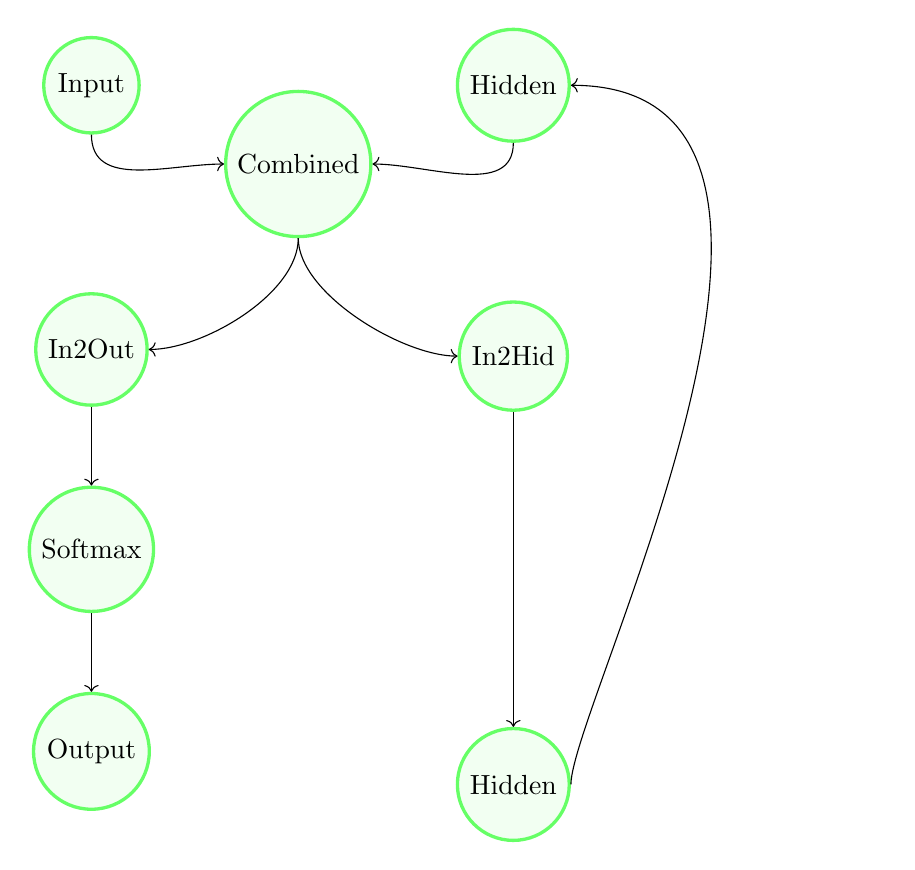
\begin{tikzpicture}[
        roundnode/.style={circle, draw=green!60, fill=green!5, very thick, minimum width={width("hidden")},}
        ]
    
        % Nodes
        \node[roundnode] (combined) {Combined};
        \coordinate[above of=combined] (ac);
        \coordinate[below of=combined] (bc);
        \node[roundnode] (input) [left=2cm of ac] {Input};
        \node[roundnode] (hidden) [right=2cm of ac] {Hidden};
        \node[roundnode] (i2o) [below=2cm of input] {In2Out};
        \node[roundnode] (i2h) [below=2cm of hidden] {In2Hid};
        \node[roundnode] (softmax) [below=1cm of i2o] {Softmax};
        \node[roundnode] (12hidden) [below=4cm of i2h] {Hidden};
        \node[roundnode] (output) [below=of softmax] {Output};
            
        % Lines
        \draw[->] (input.south) .. controls +(down:7mm) and +(left:7mm) ..  (combined.west);
        \draw[->] (hidden.south) .. controls +(down:7mm) and +(right:7mm) ..  (combined.east);
        \draw[->] (combined.south) .. controls +(down:7mm) and +(right:7mm) ..   (i2o.east);
        \draw[->] (combined.south).. controls +(down:7mm) and +(left:7mm) .. (i2h.west);
        \draw[->] (i2o.south) --  (softmax.north);
        \draw[->] (i2h.south) --  (12hidden.north);
        \draw[->] (softmax.south) --  (output.north);
        
        \draw[->] (12hidden.east) .. controls +(up:1cm) and +(right:4cm) ..  (hidden.east);
    
    \end{tikzpicture}

\end{figure}
\begin{itemize}
    \item input\textunderscore size : Input parameter of class is size of the data. Size of one-hot encoded feature vector. 
    \item  hidden\textunderscore size : Dimensionality of hidden state of the \acs{RNN} cell.
    \item  output\textunderscore size : Number of categories in which the input need to be classified.
    \item i2h : input-to-hidden, a fully connected linear layer gets the next hidden state from the current input and previous state.
    \item i2o : input-to-output,a fully connected linear layer gets the next output state from the current input and previous hidden state.
    \item softmax: Layer used for classification. 
\end{itemize}

  

% \section{Forward propagation equation} \label{sec:forward-propagation}
% The forward propagation equations for the recurrent neural network (RNN) depicted in code \ref{code:RNN-class}, assuming the tanh activation function for hidden units and a discrete output (used for predicting words or characters) \parencite{Goodfellow-et-al-2016}, are as follows
% \begin{enumerate}
%     \item Initialization: \\
%     Set initial state: $\textit{\textbf{h}}^{(0)}$ (hidden state at time $t=0$)
%     \item For each time step from $t=1$ to $t=\tau$: \\
%     \begin{align}
%         a(t) &= b + Wh(t-1) + Ux(t) \quad  \\
%         h(t) &= \tanh(a(t)) \quad  \\
%         o(t) &= c + Vh(t) \quad  \\
%         \hat{y}(t) &= \text{softmax}(o(t)) \quad 
%         \end{align}
% \end{enumerate}

% Here:
% \begin{itemize}
%   \item $x(t)$ represents the input at time step $t$.
%   \item $h(t)$ is the hidden state at time step $t$, which is updated based on the previous hidden state $h(t-1)$ and the current input $x(t)$.
%   \item $a(t)$ is the activation vector at time step $t$, computed by adding the bias vector $b$ to the weighted sum of the previous hidden state $h(t-1)$ and the current input $x(t)$, where $W$ is the weight matrix for the recurrent connections and $U$ is the weight matrix for the input connections.
%   \item $\tanh()$ is the hyperbolic tangent activation function, which squashes the values between $-1$ and $1$, introducing non-linearity to the hidden state.
%   \item $o(t)$ is the output vector at time step $t$, computed by adding the bias vector $c$ to the weighted sum of the current hidden state $h(t)$ using the weight matrix $V$.
%   \item $\hat{y}(t)$ is the normalized probability vector (predicted probabilities) over the output, obtained by applying the softmax operation to $o(t)$, which converts the unnormalized log probabilities into valid probabilities summing up to $1$.
% \end{itemize}

\clearpage

\section{Pytorch's $SoftMax$ function and its variations}

\subsection*{Softmax or normalized exponential.} \label{sec:softmax}

\begin{align}
    \text{Softmax}(x_i) = \frac{{\exp(x_i)}}{{\sum_{j=1}^n \exp(x_j)}} \label{eq:softmax}
\end{align}

\begin{itemize}
    \item Pytorch's nn.Softmax applies the Softmax function to an n-dimensional input Tensor rescaling them so that the elements of the n-dimensional output Tensor lie in the range [0,1] and sum to 1.
    \item In this representation, \(x_i\) is the \(i\)-th element of the input vector \(\mathbf{x} = [x_1, x_2, \ldots, x_n]\). The softmax function calculates the probability of the element \(x_i\) being chosen by dividing the exponential of \(x_i\) by the sum of the exponentials of all elements in the vector \(\mathbf{x}\). This calculation ensures that the resulting probabilities sum up to 1, forming a valid probability distribution over the elements in the vector \(\mathbf{x}\).
    \item The softmax function transforms a vector of logits into a probability distribution, making it useful for tasks like classification, where the model needs to make a decision based on the input data.
    \item Pytorch's nn.LogSoftmax function applies $\text{log}\left(\text{Softmax}(\mathbf{x})\right)$ to an n-dimentional input tensors. \\
\end{itemize}



% As per \parencite{Book-Bishop-Neural} the term softmax is used because this activation function represents a smooth version of the winner-takes-all activation model in which the unit with the largest input has output +1 while all other units have output 0.



\subsection*{\acf{ALL}}

\begin{itemize}
    \item Pytorch's \parencite{Paszke.03122019} nn.AdaptiveLogSoftmaxWithLoss module implements \acf{ALL}.
    \item Adaptive Softmax \parencite{Grave.14092016} is effective when large number of classes are to be handled. Traditional Softmax computation becomes computationally expensive and memory intensive if number of output classes are very high. Softmax requires calculating the exponential of the logits for each class. However, when the number of classes or labels are very high, the Softmax based classification becomes computationally expensive.
    \item Adaptive Softmax counter this issue by clustering the classes according to their frequency of occurrence. A simple strategy to reduce the overall computation time is to partition the labels \(V\) into two clusters as \(V_h\) and \(V_l\), where \(V_h\) denotes the distribution consisting of the most frequent classes, and where \(V_l\) are many rare classes. The classifier frequently accesses \(V_h\), which motivates the fact that it should be computed efficiently. In contrast,  \(V_l\) less frequently, and the corresponding computation can be slower. This suggests defining clusters with unbalanced cardinalities \(|V_h| \geq |V_l|\) and probabilities \(P(V_h) \geq P(V_t)\).
\end{itemize}










\section{Summary}

In this chapter, author describes how he ideated the concept of vocabulary based RNN. This method is a modified version of character level RNN \parencite{sean}. The method of converting the product name into a tensor format is described in this chapter. 

Architecture of the RNN and pictorial representation of flow of data within the neural network is depicted. The chapter gives an overview of the activation functions and forward propagation method. The code snippet of the defining architecture of \acl{RNN} class is given along with its explaination.  

In this chapter, Pytorch's loss functions such as  SoftMax, LogSoftMax, Adaptive Softmax and its equivalent mathematical  representations is described. 
\include{chapters/training-hypertuning}
\chapter{Mathematical Foundations of Classification Model}



\section{Probability Distribution}

A probability distribution is the information of how likely a random variable or set of variables is to take each of its possible states. The way the probability distribution is described depended on whether the variables are discrete (finite set of variables) or continuous \parencite[Page 54]{Goodfellow-et-al-2016}. 

In this paper, the finite number of categories to be predicted indicate that the probability distribution variable is of discrete type.  The probability that variable $X = x$ is denoted by $ P(x) $, with a probability of 1 indicating that $x-x$ is certain and probability of 0 indicating an impossible event \parencite[Page 55]{Goodfellow-et-al-2016}.


The probability values ranging between 0  and 1 are called \acf{PMF} denoted as $ P $. To ensure that \acs*{PMF} provides valid probabilities the function $P$ must satisfy following propertise.


\begin{itemize}
    \item Domain of PMF must be defined for all possible states of random variable $x$. It should specify probabilities for each value $x$. For example, of the variable of vector representation of product name ``X'' the $P$ must be defined for all categories.
    \item The $ P(x) $ must satisfy $0 \leq  P(x) \leq  1$.
    \item Impossible events have probability 0.
    \item Certain events have probability 1.
    \item Normalization property indicating sum of all probabilities equals to 1.
\end{itemize}


\begin{table}[H]
    \centering
    \begin{tabular}{ccccccc}
        \hline
        $x$ & $x_1$ & $x_2$ & $x_3$ & $\dots$ & $x_n$ \\
        \hline
        $P(x)$ & $P_1$ & $P_2$ & $P_3$ & $\dots$ & $P_n$ \\
        \hline
    \end{tabular}
    \caption{Probability Distribution $P(x)$ for Random Variable $x$}
    \label{tab:probability-distribution}
\end{table}

where \(P_i > 0\), \(i=1\) to \(n\) and \(P_1 + P_2 + P_3 + \ldots + P_n =1\) \\
\chapter{Building a Knowledge graph} \label{sec:building-kg}

Graph-based knowledge representation has been researched for decades.
A \acf{kg} acquires and integrates information into an ontology and applies a reasoner to derive new knowledge \parencite{LisaEhrlinger}.
The knowledge base is a dataset with formal semantics that can contain different kinds of knowledge, for example, rules, facts, axioms, definitions, statements, and primitives \parencite{Davies.2008cop.2006}.

\begin{figure}[h!]
    \centering
    \includesvg[scale=0.5]{Thesis_kg.svg}
    \caption{\acl{kg} architecture}
    \label{fig:kg}
    \parencite[Chapter 4]{LisaEhrlinger}
\end{figure}

Figure \ref{fig:kg} illustrates the processing of plain text from various sources such as  Wikipedia API, PDF into a graph. This abstract architecture represented by \Citeauthor{LisaEhrlinger} of a \acl{kg} portraits the assumption that a \acl{kg} is more than a \acf{kb}. \acl{kg} is a combination of \acl{kb} and \acf{qe}. 

\Iac{qe} is a set of graph of possible questions that could be formed in reference to \iac{kb}. \acf{qg} for comprehensive reading is a challenging task. There are datasets available for  \acs{qg}, one of it is Stanford Question Answering Dataset v1.0 (SQuAD) consisting of questions posed by crowd workers on a set of Wikipedia articles \parencite{PranavRajpurkar.}. The limitation with such a data set is that these do not contain unanswerable questions. Building a machine learning model when no answer is supported was out of scope of SQuAD objective \parencite{LupeHernandez}.  Study on automatic question generation from an attention-based sequence learning model \parencite{Vaswani.12062017} for  \ac{qg} and investigate the effect of encoding sentence- vs. paragraph-level information \parencite{DuXinya.29042017}, reduces reliance on handcrafted rule based systems.

\clearpage

\section{Fetching text corpus}


One of the first things required for \acf*{nlp} tasks is a creating a text corpus.
In linguistics and \acs{nlp}, corpus refers to a collection of texts. An intriguing application of knowledge graphs within the e-commerce industry involves the creation of a comprehensive information network concerning products. Such a knowledge graph can serve as the basis for chatbots to provide answers to user queries. Converting unstructured text corpus into a directed acyclic graph. Knowledge base serve as a foundation for chatbot applications to traverse through the graph
structure, locate relevant leafs nodes, and formulate human-readable response.


Wikipedia\footnote{https://www.wikipedia.org/} is primarily an encyclopedia with the additional benefit of heavy linking between articles and without the size constraints of paper articles \parencite{TorstenZesch}. 

\section{spaCy - Dependency Parsing} \label{dependencyparsing}

spaCy \parencite{spacy2} features neural models for parsing and entity recognition. These models can be trained for \acf{ner} , tagging and parsing. Its official page on usage\footnote {https://v2.spacy.io/usage/} provides in-depth code example for information extraction.

In figure \ref{fig:dp}, we see a complex sentence's dependency parsing. It has a \acf{nsubj}, connecting \acfp{pobj} with \acfp{adp} and no \acf{dobj}.

\begin{figure}[htp!]
    \centering    
    \includesvg[scale=0.16]{dependency-parser.svg}
    \caption{Navigating the parse tree and subtrees}
    \label{fig:dp}
\end{figure}

The \acs{nsubj} "oil", itself does not give a complete meaning. However, upon combining its dependency noun "Motor", which is "Motor oil"  gives us an understanding of the topic. Traversing from \acs{nsubj} to  \acfp{conj} provides us with three related compound nouns belonging to a similar group.

"Motor oil", "Engine Oil", "Engine Lubricant"

Traversing further right of the dependency tree we can extract the \acsp{pobj}.  An \acf{amod} "internal" is connecting compound noun "combustion engine".

\section{Knowledge graph with Networkx}

The directed graphs created with Networkx \parencite{hagberg2008exploring} is suitable for representing dependency parsing of a sentence mentioned in section \ref{dependencyparsing}. A knowledge base are represented as triples of \acf{SRO}. In which the subject and object are nodes are entities of a graph and relation are directed edges or links between the nodes.

\subsection{What to use as nodes n(x) and edges e(y)?}

In table \ref{table:1}, distingution of triples by  \acs{POS} tags is depicted. 
\begin{table}[h!]
\begin{center}
\begin{tabular}{>{$}l<{$} l}

triples   &   \acf{POS} tags   \\
\hline
n(subject)   &   \acs{nsubj} , \acs{pron}                          \\
n(object)  &   \acs{dobj}    , \acs{pobj}                     \\
e(relation)  &   \acs{adp}, verb
\end{tabular}
\end{center}
\caption{\acs{SRO} and \acs{POS} tags mappings}
\label{table:1}
\end{table}

\section{Summary}


In this chapter, using the dependency parsing of an unstructured sentence, building a knowledge graph is proposed.  The process involves textual information on a product from various sources pass through various methods such as dependency parsing, part of speech tagging, named entity relationship mapping. The processed text is created into a directed graph along with the question engine is called the knowledge graph.  

Further research has to be conducted on generating knowledge graph. As per \parencite{LisaEhrlinger}, there are limitations with knowledge graphs as comprehensive reading is a challenging task.
\chapter{Conclusion and Outlook}


\section{Answer to Research Questions}
\begin{enumerate}[label=\textbf{RQ\arabic*:}]
    \item What are the use cases in which natural language processing and machine learning model can be utilized in an E-Commerce industry?
    
    Machine learning model can generate well-defined product taxonomy. Author introduces a methodology for such a model in section \ref{sec:ideate}. A well-defined product taxonomy is the foundation for many use cases like the ones listed below:
        \begin{itemize}
        \item Product recommendation system.
        
        The machine learning model can classify and recommend products from the wide range of products to the customer based on the customer's transaction history. The transaction history containing product relevance feedback such as click ``clicks'', ``cart-adds'', ``orders'', ``revenue'' \parencite{KarmakerSantu.2017} are usable if the taxonomy is well-defined. 
        
        \item Search bar autocompletion.
        
        A lot of research has been conducted in the field of user experience in terms of product search. A facet in user interface is an extended drop down menu with filtered result set. \parencite{Tagliabue.26052020} proposes a real time personalized catalog generation by combining customer search logs and in-session data. 
        
        \item Customer conversational shopping.
            
        \Parencite{ChrisMessina} states that gradually traditional commerce will shift towards conversational commerce. An experience of shopping on the go or hands-free assistance could be trending. Major Ecommerce  industries offering voice assistance devices includes feature of buying products on voice command.  


        \item Building a knowledge graph based on the textual details of a product. Refer section \ref{sec:building-kg}
        \item Virtual customer support chatbot may leverage the knowledge graph to answer queries raised by customers.
    \end{itemize}
    
    \item For a product classification task, how to define product features as an input for machine learning model?
    
   Based on the level of product taxonomy the number of features may vary. Table \ref{table:feature_decription} lists some features are listed simply by prior knowledge of the product domain. However, section \ref{sec:feature-selection} describes various methods to reduce dimensionality.

    
    \item How does a machine learn pattern in product features for classification?
    

    \begin{enumerate}[label=\textbf{SRQ\arabic*:}]
        \item What are the mathematical equations behind the learning process?
    
        Author has dedicated Chapter \ref{ch:math-behid} for step by step illustration of learning process. Author begins the chapter with basic mathematical representation of a neural network, followed by equations for feedforward, back-propagation. Further, author describes the probability distribution and its relation with the project in this paper. What is the role of partial derivatives to reduce the loss function is described.  
        \item What are the mathematical reasons for applying certain pytorch functions during the training process? 
        
        Section \ref{sec:Logsoft} describes mathematical reasons behind using Pytorch's functions such as LogSoftMax. Chapter \ref{ch:math-behid} is detailed with the explanation of applying log to a value.         

    \end{enumerate}
    
    \item What is the algorithm to train the machine learning model to predict the product taxonomy?
        
    Author modified the algorithm of \parencite{sean}   classifying names with character-level RNN. Instead of series of tensor representation of characters, author use tensor representation of features. The RNN model learns the pattern and predicts the product taxonomy.

  \end{enumerate}

  \section{Future scope}

  In this paper, author has researched on the machine learning task to text based classification. Research has been conducted on use cases of text based classification in E-Commerce. Author limited the research surrounding basic understanding of neural network, its mathematical equations, creating a model which predicts product taxonomy.  This paper is also a guide for individual who seek basic understanding of machine learning as well as overview of product taxonomy and its importance in E-commerce.

  There is a scope of research on image classification and its use cases in the E-commerce industry. Images are vital component of an E-commerce website. There is saying ``A picture is worth a thousand words''. The product image itself has so much information  to be tapped. 

  Few of them are listed below:
  \begin{itemize}
    \item Image captioning.
    
    Generating text from the image is a useful process in E-commerce. For example, product image also describes its features such as color. Such information can be added to the caption of the image. \parencite[Section 15.4.7]{pml1Book} describes an example of image captioning using the sequential data processing network with \textbf{attention algorithm}.
    
    \item Attention based image classification.
    
    \parencite{Vaswani.12062017} proposes a network architecture named Transformers which uses attention in the encoder and decoder in the machine translation tasks. Using the transformer model to process the sequence of pixels in a product image to identify the clustered components or to identify which other product could be a part of the product.
    For example, image from Appendix B figure \ref{fig:sparepart} is product image, using attention based image classification, identifying the products which fit in and around the processed product image could enable E-Commerce industries cluster the products.
 


    \item Image based categorization.
    
    A Machine learning model can generate product taxonomy based on the image of the product. Clustering the products based on the image could also enable to define a better product taxonomy. 

    \item Image to image translation.
   
    Using \acfp{GAN} \parencite{Goodfellow.31122016}, a sketch can be converted to photorealistic image.     
    

  \end{itemize}

\pagenumbering{roman}
\pagestyle{mypagestyle}

% Add the List of Figures to the table of contents
\cleardoublepage % Ensure the correct page
\addcontentsline{toc}{chapter}{\listfigurename}
\listoffigures


\addcontentsline{toc}{chapter}{\listtablename}
\listoftables

\lstlistoflistings


\clearpage
% \printglossary[type=\acronymtype]

% \printglossary
\addcontentsline{toc}{chapter}{Bibliography}


\nocite{*}
\printbibliography[title={References}]



% \defbibheading{bibempty}{}

% \let\oldbib\thebibliography
% \let\endoldbib\endthebibliography
% \renewenvironment{thebibliography}
%   {\vspace{\baselineskip}\begin{oldbib}}
%   {\end{oldbib}\vspace{\baselineskip}}

\addcontentsline{toc}{chapter}{Appendices}
\appendix


\begin{appendices}

\chapter*{Appendices}
\addcontentsline{toc}{chapter}{Appendices}
% Additional appendices can be added here
\section{List of Abbreviations}
% \newacronym{kgs}{KGs}{Knowledge Graphs}
% \newacronym{nlp}{NLP}{Natural Language Processing}
% \acro{ecu}[ECU]{European currency unit}
% \begin{acronym}[ECU]


% \chapter*{List of abbreviations} \label{LOA}
\begin{acronym}
\acro{kg}[KG]{Knowledge graph}
\acro{kb}[KB]{Knowledge base}
\acro{qe}[QE]{Questioning Engine}
\acro{nlp}[NLP]{Natural Language Processing}

\acro{qg}[QG]{Question generation}

\acro{ner}[NER]{Named Entity Recognition}
\acro{adp}[adp]{adposition}
\acro{pobj}[pobj]{prepositional object}
\acro{dobj}[dobj]{direct object}
\acro{nsubj}[nsubj]{nominal subject}
\acro{conj}[conj]{coordinating conjunction}
\acro{amod}[amod]{adjectival modifier}
\acro{POS}[POS]{part of speech}
\acro{pron}[pron]{pronoun}
\acro{SRO}[SRO]{subject,relation and object}
\acro{Tf-Idf}[Tf-Idf]{Term frequency-Inverse document frequency}
\acro{Tf}[Tf-Idf]{Term frequency}
\acro{Idf}[Idf]{Inverse document frequency}
\acro{KNN}[KNN]{\textit{k} -Nearest Neighbors}
\acro{RNN}[RNN]{Recurrent Neural Network}
\acro{ALL}[ALL]{Adaptive LogSoftmax with Loss}
\acro{NLLLoss}[NLLLoss]{Negative log likelihood loss}
\acro{BPTT}[BPTT]{Back Propagation through time}
\acro{DAG}[DAG]{directed acyclic graph }
\acro{SGD}[SGD]{Stochastic gradient descent }
\acro{CLR}[CLR]{Cyclic learning rate }
\acro{LTR}[LTR]{Learn to Rank }
\acro{IR}[IR]{Information Retrieval }
\acro{AI}[AI]{Artificial Intelligence }
\acro{PMF}[PMF]{Probability Mass Function }
\acro{MSE}[MSE]{Mean Squared Error}
\acro{GAN}[GAN]{generative adversarial network}
\acro{PIM}[PIM]{Product Information Management}
\acro{SKU}[SKU]{stock-keeping unit}

\end{acronym}


\section{Appendix A}
For this project, python client elasticsearch 6.8.2 is installed as the client needs to be compatible with Elastic search version being used. The official Python client provides mapping with Elasticsearch REST APIs.

\begin{lstlisting}[language=Python,caption={Elastic search},label={code:es_search}]
    resp=self.es.search("english-name-category",{"_source":["id","name","category"],
    'from':_from,
    'size' :_size ,
    "query": {"match_all": {}}})
    \end{lstlisting}
% Content for Appendix A goes here...

\subsection*{Confusion matrix}
\begin{lstlisting}[language=Python,caption={Confusion matrix},label={code:confusion matrix}]
def confusionMatix(self,df_en):
# Keep track of correct guesses in a confusion matrix
data = Data(df_en)
n_categories = len(data.all_category)

batch = random.choices(data.all_category,k=20)

confusion = torch.zeros(n_categories, n_categories)
n_confusion = 10000

# Go through a bunch of examples and record which are correctly guessed
for i in range(n_confusion):
    category, name, category_tensor, name_tensor = data.randomTrainingExample()
    if category in batch:
        output = self.evaluate(name_tensor)
        guess, guess_i = data.categoryFromOutput(output)
        category_i =data.all_category.index(category)
        confusion[category_i][guess_i] += 1

# Normalize by dividing every row by its sum
for i in range(20):
    confusion[i] = confusion[i] / confusion[i].sum()


# Set up plot
fig = plt.figure()
ax = fig.add_subplot(111)
cax = ax.matshow(confusion.numpy())
fig.colorbar(cax)

# Set up axes
ax.set_xticklabels([''] + data.all_category, rotation=45)
ax.set_yticklabels([''] + data.all_category)

# Force label at every tick
ax.xaxis.set_major_locator(ticker.MultipleLocator(1))
ax.yaxis.set_major_locator(ticker.MultipleLocator(1))

# sphinx_gallery_thumbnail_number = 2
plt.show()
plt.savefig('confusion.png', dpi=400)

\end{lstlisting}

\subsection*{Load PyTorch model}
\begin{lstlisting}[language=Python,caption={Load PyTorch model},label={code:Loadpt}]
class Predict():
    def __init__(self):
         self.rnn = torch.load('ngram-rnn-classification.pt')
        \end{lstlisting}
\clearpage
\section{Appendix B}
\begin{figure}[H]
    \centering    
    \includegraphics[scale=0.5]{ht_rm.jpg}
    \caption{Hydraulic filter automatic transmission VAICO V70-0613 for Lexus RX \parencite{RM}}
    \label{fig:sparepart}
\end{figure}

\end{appendices}


\end{document}